% Agent State Machine TikZ Diagram
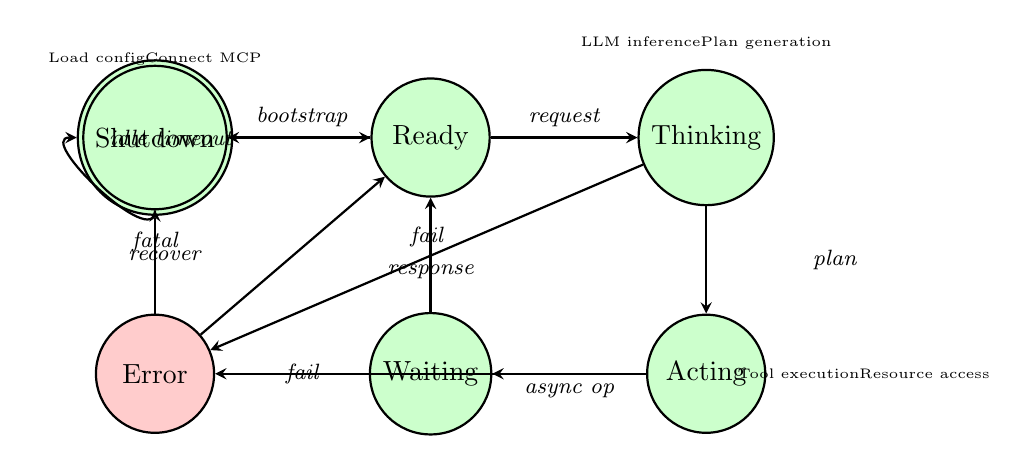
\begin{tikzpicture}[
    node distance=2cm,
    auto,
    state/.style={
        circle,
        draw,
        fill=green!20,
        thick,
        minimum size=1.5cm,
        align=center
    },
    error/.style={
        circle,
        draw,
        fill=red!20,
        thick,
        minimum size=1.5cm,
        align=center
    },
    arrow/.style={
        ->,
        thick,
        >=stealth
    },
    label/.style={
        font=\footnotesize\itshape,
        text width=3cm,
        align=center
    }
]

% States
\node [state] (init) {Initializing};
\node [state, right of=init, node distance=3.5cm] (ready) {Ready};
\node [state, right of=ready, node distance=3.5cm] (thinking) {Thinking};
\node [state, below of=thinking, node distance=3cm] (acting) {Acting};
\node [state, left of=acting, node distance=3.5cm] (waiting) {Waiting};
\node [error, left of=waiting, node distance=3.5cm] (error) {Error};
\node [state, above of=error, node distance=3cm] (shutdown) {Shutdown};

% Transitions
\draw [arrow] (init) -- node[above, label] {bootstrap} (ready);
\draw [arrow] (ready) -- node[above, label] {request} (thinking);
\draw [arrow] (thinking) -- node[right, label] {plan} (acting);
\draw [arrow] (acting) -- node[below, label] {async op} (waiting);
\draw [arrow] (waiting) -- node[below, label] {response} (ready);
\draw [arrow] (thinking) -- node[above, label] {fail} (error);
\draw [arrow] (acting) -- node[left, label] {fail} (error);
\draw [arrow] (ready) -- node[left, label] {idle timeout} (shutdown);
\draw [arrow] (error) -- node[left, label] {recover} (ready);
\draw [arrow] (error) -- node[above, label] {fatal} (shutdown);
\draw [arrow] (shutdown) to[out=270,in=180] (init);

% Annotations
\node [above of=init, node distance=1cm, font=\tiny] {
    Load config\\
    Connect MCP
};

\node [above of=thinking, node distance=1.2cm, font=\tiny] {
    LLM inference\\
    Plan generation
};

\node [right of=acting, node distance=2cm, font=\tiny] {
    Tool execution\\
    Resource access
};

\end{tikzpicture}
